\begin{figure}[H]
  \centering
  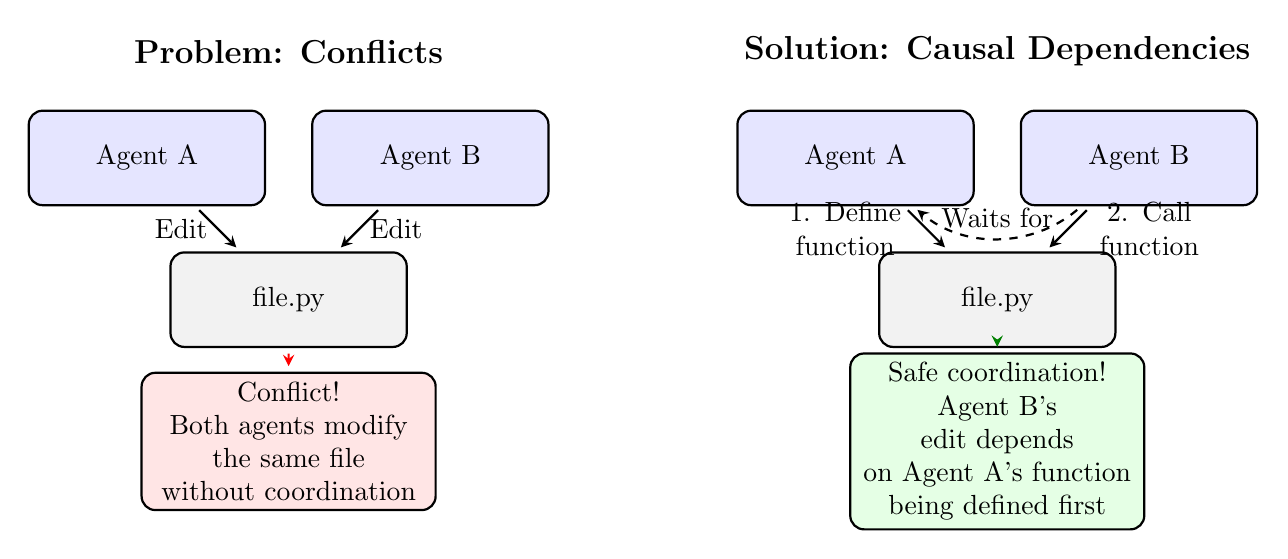
\begin{tikzpicture}[
    scale=0.9,
    box/.style={draw, minimum width=3cm, minimum height=1.2cm, align=center, rounded corners=5pt, thick},
    agent/.style={box, fill=blue!10},
    file/.style={box, fill=gray!10},
    problem/.style={draw, fill=red!10, text width=3.5cm, align=center, rounded corners=5pt, thick},
    solution/.style={draw, fill=green!10, text width=3.5cm, align=center, rounded corners=5pt, thick},
    arrow/.style={->, >=stealth, thick, shorten >=2pt, shorten <=2pt},
    dashedarrow/.style={->, >=stealth, thick, dashed, shorten >=2pt, shorten <=2pt}
  ]

  % Problem side (left) - increased horizontal spacing
  \node[draw=none, font=\large\bfseries] at (-5,3.5) {Problem: Conflicts};

  \node[agent] (agent_a1) at (-7,2) {Agent A};
  \node[agent] (agent_b1) at (-3,2) {Agent B};

  \node[file] (file1) at (-5,0) {file.py};

  \draw[arrow] (agent_a1) -- node[left] {Edit} (file1);
  \draw[arrow] (agent_b1) -- node[right] {Edit} (file1);

  \node[problem] (conflict) at (-5,-2) {Conflict!\\Both agents modify\\the same file\\without coordination};
  \draw[arrow, red, thick] (file1) -- (conflict);

  % Solution side (right) - increased horizontal spacing
  \node[draw=none, font=\large\bfseries] at (5,3.5) {Solution: Causal Dependencies};

  \node[agent] (agent_a2) at (3,2) {Agent A};
  \node[agent] (agent_b2) at (7,2) {Agent B};

  \node[file] (file2) at (5,0) {file.py};

  \draw[arrow] (agent_a2) -- node[left, align=center, text width=1.8cm] {1. Define\\function} (file2);
  \draw[arrow] (agent_b2) -- node[right, align=center, text width=1.8cm] {2. Call\\function} (file2);

  \draw[dashedarrow, bend left=40] (agent_b2) to node[above] {Waits for} (agent_a2);

  \node[solution] (solution) at (5,-2) {Safe coordination!\\Agent B's edit depends\\on Agent A's function\\being defined first};
  \draw[arrow, green!50!black, thick] (file2) -- (solution);

  \end{tikzpicture}
  \caption{Causal Dependency Management: On the left, we see the problem when multiple agents edit the same file without coordination, leading to conflicts. On the right, Arc's solution uses causal dependencies to ensure that operations happen in the correct order - Agent B waits for Agent A to define a function before trying to call it.}
  \label{fig:causal_dependency}
\end{figure}
